\documentclass[10pt,a4paper]{article}
\usepackage[margin=2cm]{geometry}
\usepackage[T1]{fontenc}
\usepackage{lmodern}
\usepackage{graphicx}
\usepackage{xcolor}
\usepackage{booktabs}
\usepackage{tabularx}
\usepackage{float}
\usepackage[font=small,labelfont=bf]{caption}
\usepackage{subcaption}
\usepackage{listings}
\usepackage{pdflscape}
\usepackage{fancyhdr}
\usepackage{needspace}
\usepackage{tikz}
\usetikzlibrary{arrows.meta,positioning,calc}
\usepackage[hidelinks]{hyperref}

\setlength{\headheight}{14pt}
\setlength{\parskip}{0.5em}
\setlength{\parindent}{0pt}
\renewcommand{\arraystretch}{1.12}
\pagestyle{fancy}\fancyhf{}
\fancyhead[L]{femtoRV32, Milestone 3}\fancyhead[R]{CSCE 3301, Fall 2026}\fancyfoot[C]{\thepage}
\lstset{basicstyle=\ttfamily\scriptsize,breaklines=true,frame=single,columns=fullflexible}
\newcommand{\sig}[1]{\texttt{\detokenize{#1}}}
\newcommand{\file}[1]{\texttt{\detokenize{#1}}}
\newcommand{\hd}[1]{\needspace{8\baselineskip}\vspace{0.4em}{\large\bfseries\color{blue!40!black}#1}\par\vspace{-0.2em}\hrule\vspace{0.4em}}

\begin{document}

\begin{center}
{\Huge\bfseries femtoRV32}\\[0.3em]
{\Large Pipelined RV32IM processor with a single single-ported memory}\\[0.3em]
Design, implementation and verification report, 19 November 2026\\[0.5em]
Kareem Abdellatif, Mohamed AboElfotouh, Mostafa Fayed\\
Bonus features: Bonus 2 (RV32M) and Bonus 4 (branch resolution in ID)
\end{center}

\hd{1. Datapath architecture}

Instructions and data share one single-ported, byte-addressable memory. One instruction is issued every two clock cycles (CPI = 2), so the memory port is never needed twice in the same cycle. Each instruction takes six cycles in three stages of two cycles (C0, C1):

\begin{center}\small
\begin{tabularx}{0.95\linewidth}{@{}l X X@{}}
\toprule
Stage & C0 & C1\\
\midrule
0 & IF: fetch at PC (memory port) & ID: decode, register read, branch/jump decision\\
1 & EX: ALU & MEM: load / store (memory port)\\
2 & WB: register file write & unused\\
\bottomrule
\end{tabularx}
\end{center}

Figure~\ref{fig:datapath} shows the datapath. A one-bit toggle (\file{PhaseController.v}) gives the enables \sig{isC0} and \sig{isC1}; every register is on one clock and loads only on its enable (IF\_ID and EX\_MEM in C0, ID\_EX and MEM\_WB in C1). In C0 the memory address is the PC and in C1 it is the EX\_MEM result.

\textbf{Hazards.} When an instruction is in ID, the instruction before it is in MEM and the one before that was written back in the previous C0 (the register file is written in C0 and read in C1). One forwarding unit in ID therefore suffices: it takes the value of the instruction in MEM from the EX\_MEM result, or from the memory output of the same C1 if that instruction is a load. The pipeline never stalls, including for load-use.

\textbf{Branches (Bonus 4).} Branch condition and the branch, JAL and JALR targets are computed in ID. The PC loads the target at the end of that C1 and the next fetch is already correct, so a taken branch loses no cycle and no wrong-path instruction is fetched.

\textbf{EBREAK / NOPs.} EBREAK sets a halt flip-flop (the PC never changes again). ECALL, FENCE, FENCE.TSO and PAUSE are NOPs.

\begin{landscape}
\begin{figure}[p]
\centering
\resizebox{\linewidth}{!}{% Datapath schematic of the 3-stage, 6-cycle femtoRV32 (pipeline.v).
% A label next to a short arrow ("tag") is wired to the tag with the same
% name elsewhere in the drawing; this keeps the drawing free of long wires.
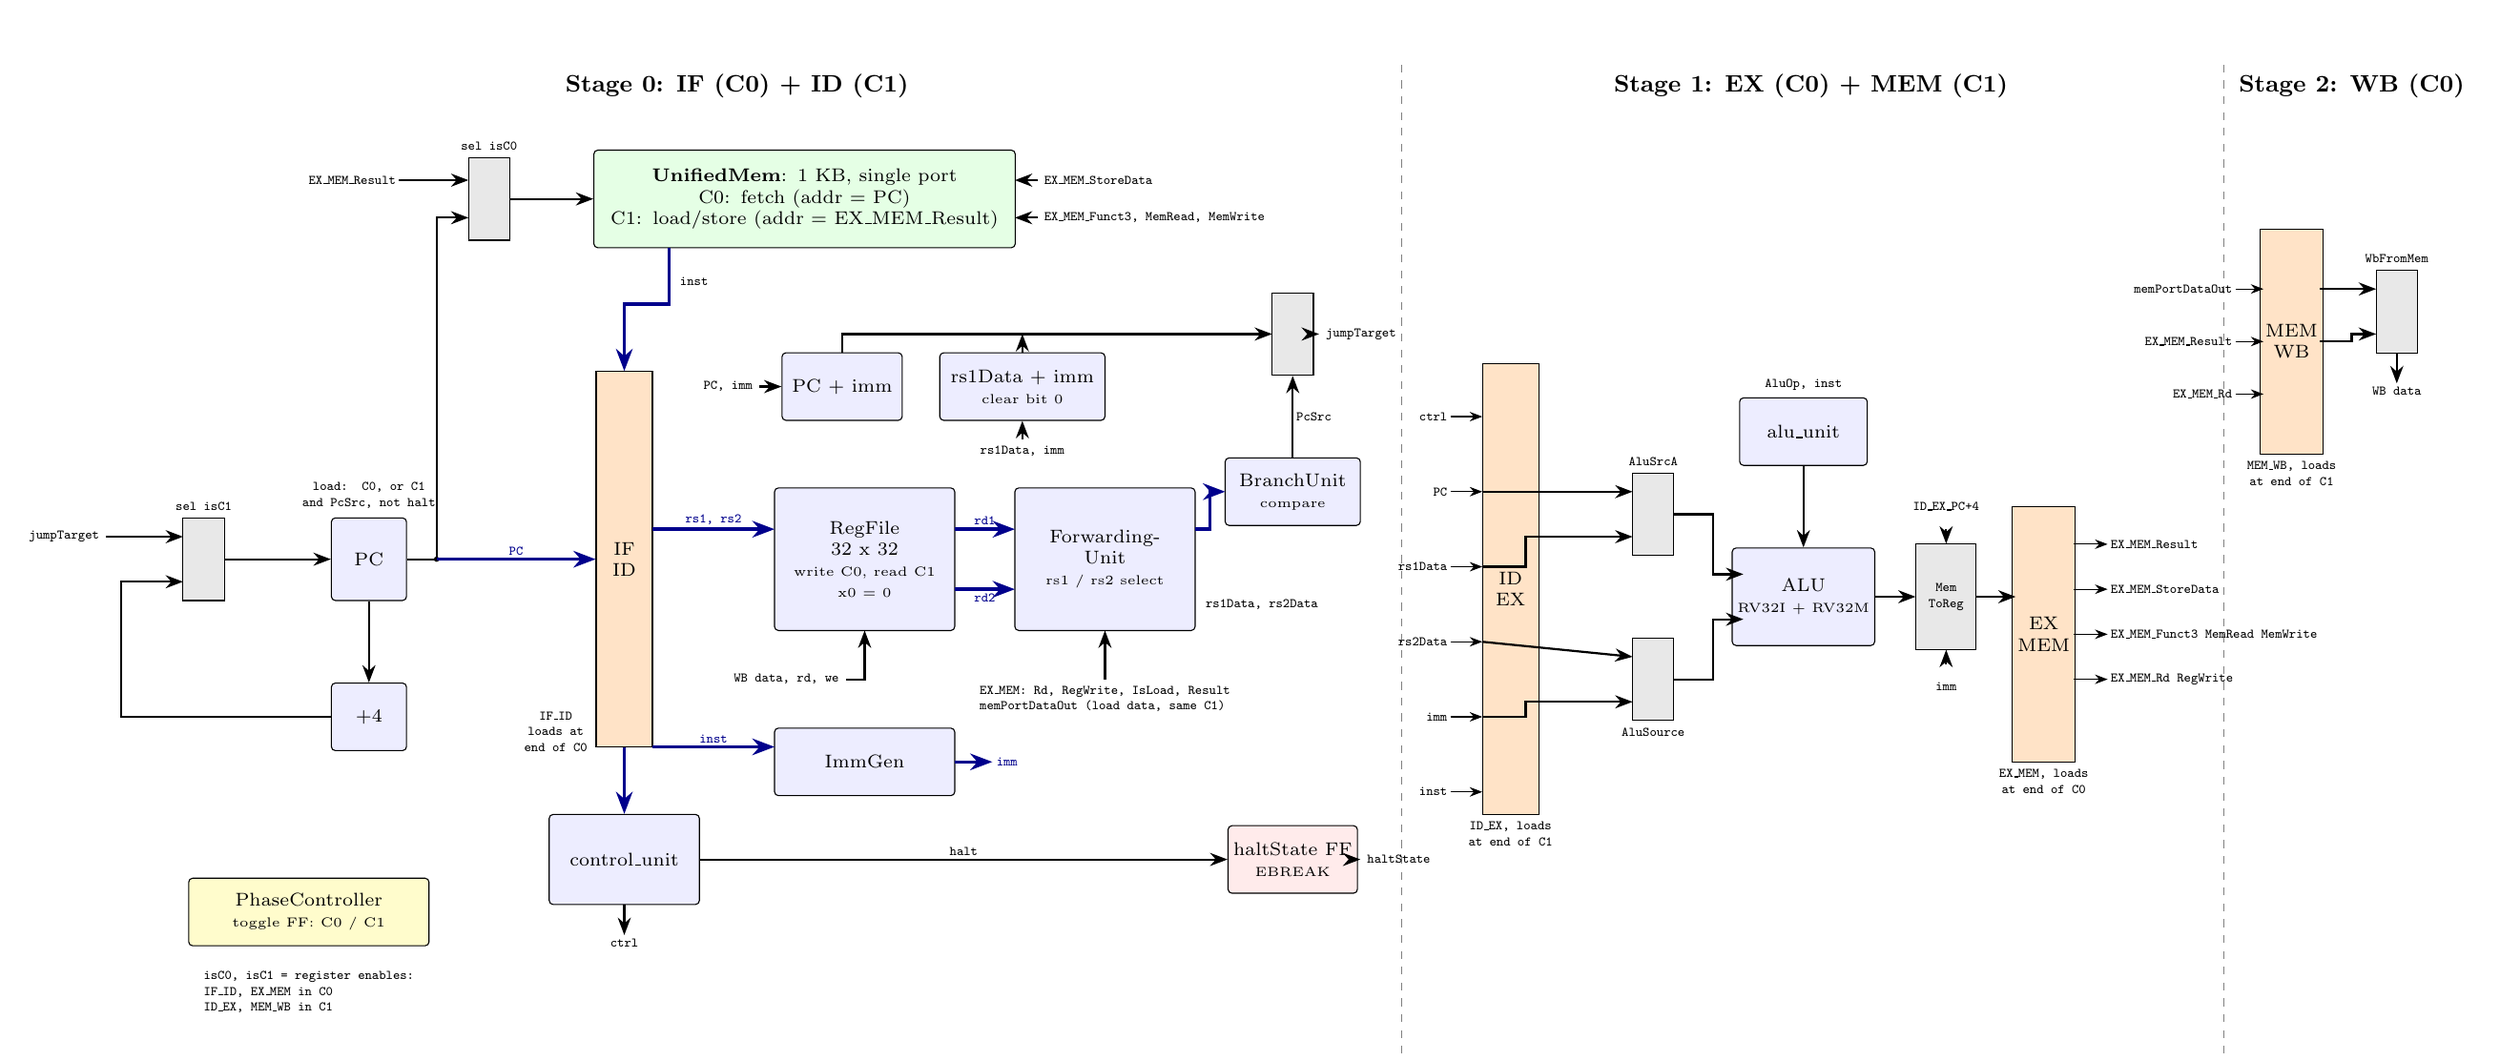
\begin{tikzpicture}[
  x=1cm,y=1cm,
  font=\scriptsize,
  >=Stealth,
  blk/.style={draw,rounded corners=1.5pt,fill=blue!7,align=center,minimum height=0.9cm,inner sep=2pt},
  reg/.style={draw,fill=orange!22,align=center,minimum width=0.75cm,inner sep=2pt},
  mux/.style={draw,fill=gray!18,minimum width=0.55cm,minimum height=1.1cm,inner sep=0pt},
  mem/.style={draw,rounded corners=1.5pt,fill=green!10,align=center,minimum height=1.3cm,inner sep=3pt},
  wire/.style={->,thick},
  bus/.style={->,very thick,blue!55!black},
  tag/.style={font=\tiny\ttfamily,inner sep=1pt,align=center},
  stage/.style={dashed,gray}
]
% ------------------------------------------------------------------ stages
\draw[stage] (16.35,-0.8) -- (16.35,12.6);
\draw[stage] (27.3,-0.8) -- (27.3,12.6);
\node[font=\small\bfseries] at (7.5,12.3) {Stage 0: IF (C0) + ID (C1)};
\node[font=\small\bfseries] at (21.8,12.3) {Stage 1: EX (C0) + MEM (C1)};
\node[font=\small\bfseries] at (29.0,12.3) {Stage 2: WB (C0)};

% --------------------------------------------------------------------- IF
\node[mux] (pcmux) at (0.4,6.0) {};
\node[tag,above=0.05cm of pcmux] {sel isC1};
\node[blk,minimum width=1.0cm,minimum height=1.1cm] (pc) at (2.6,6.0) {PC};
\node[tag,above=0.08cm of pc] {load: C0, or C1\\and PcSrc, not halt};
\node[blk,minimum width=1.0cm] (p4) at (2.6,3.9) {+4};
\draw[wire] (pcmux.east) -- (pc.west);
\draw[wire] (pc.south) -- (p4.north);
\draw[wire] (p4.west) -- (-0.7,3.9) -- (-0.7,5.7) -- (0.125,5.7);
\node[tag,anchor=east] at (-0.95,6.3) {jumpTarget};
\draw[wire] (-0.9,6.3) -- (0.125,6.3);

\node[mux] (amux) at (4.2,10.8) {};
\node[tag,above=0.05cm of amux] {sel isC0};
\node[mem,minimum width=5.6cm,text width=5.4cm] (mem) at (8.4,10.8) {\textbf{UnifiedMem}: 1 KB, single port\\
  C0: fetch (addr = PC)\\C1: load/store (addr = EX\_MEM\_Result)};
\draw[wire] (pc.east) -- (3.5,6.0) -- (3.5,10.55) -- (3.925,10.55);
\fill (3.5,6.0) circle (1pt);
\node[tag,anchor=east] at (3.0,11.05) {EX\_MEM\_Result};
\draw[wire] (3.0,11.05) -- (3.925,11.05);
\draw[wire] (amux.east) -- (mem.west);
\node[tag,anchor=west] at (11.55,11.05) {EX\_MEM\_StoreData};
\node[tag,anchor=west] at (11.55,10.55) {EX\_MEM\_Funct3, MemRead, MemWrite};
\draw[wire] (11.5,11.05) -- (11.2,11.05);
\draw[wire] (11.5,10.55) -- (11.2,10.55);

\node[reg,minimum height=5.0cm] (ifid) at (6.0,6.0) {IF\\ID};
\node[tag,anchor=east] at (5.55,3.7) {IF\_ID\\loads at\\end of C0};
\draw[bus] (6.6,10.15) -- (6.6,9.4) -- (6.0,9.4) -- (ifid.north);
\node[tag,anchor=west] at (6.7,9.7) {inst};
\draw[bus] (3.5,6.0) -- (ifid.west) node[midway,above,tag] {PC};

% --------------------------------------------------------------------- ID
\node[blk,minimum width=2.4cm,minimum height=1.9cm] (rf) at (9.2,6.0) {RegFile\\32 x 32\\{\tiny write C0, read C1}\\{\tiny x0 = 0}};
\node[blk,minimum width=2.4cm] (imm) at (9.2,3.3) {ImmGen};
\node[blk,minimum width=2.0cm,minimum height=1.2cm] (ctl) at (6.0,2.0) {control\_unit};
\draw[bus] (6.375,6.4) -- (8.0,6.4) node[midway,above,tag] {rs1, rs2};
\draw[bus] (6.375,3.5) -- (8.0,3.5) node[midway,above,tag] {inst};
\draw[bus] (6.0,3.5) -- (ctl.north);
\draw[bus] (10.4,3.3) -- (10.9,3.3) node[tag,anchor=west] {imm};
\draw[wire] (ctl.south) -- ++(0,-0.4) node[tag,anchor=north] {ctrl};
\node[tag,anchor=east] at (8.9,4.4) {WB data, rd, we};
\draw[wire] (8.95,4.4) -- (9.2,4.4) -- (9.2,5.05);

\node[blk,minimum width=2.4cm,minimum height=1.9cm] (fwd) at (12.4,6.0) {Forwarding-\\Unit\\{\tiny rs1 / rs2 select}};
\draw[bus] (10.4,6.4) -- (11.2,6.4) node[midway,above,tag] {rd1};
\draw[bus] (10.4,5.6) -- (11.2,5.6) node[midway,below,tag] {rd2};
\node[tag,anchor=north,align=left] at (12.4,4.35) {EX\_MEM: Rd, RegWrite, IsLoad, Result\\memPortDataOut (load data, same C1)};
\draw[wire] (12.4,4.4) -- (12.4,5.05);
\node[blk,minimum width=1.8cm] (br) at (14.9,6.9) {BranchUnit\\{\tiny compare}};
\draw[bus] (13.6,6.4) -- (13.8,6.4) -- (13.8,6.9) -- (14.0,6.9);
\node[tag,anchor=west] at (13.7,5.4) {rs1Data, rs2Data};
\node[blk,minimum width=1.6cm] (tadd) at (8.9,8.3) {PC + imm};
\node[tag,anchor=east] at (7.75,8.3) {PC, imm};
\draw[wire] (7.8,8.3) -- (tadd.west);
\node[blk,minimum width=2.2cm] (jadd) at (11.3,8.3) {rs1Data + imm\\{\tiny clear bit 0}};
\node[tag,anchor=north] at (11.3,7.55) {rs1Data, imm};
\draw[wire] (11.3,7.6) -- (jadd.south);
\node[mux] (tmux) at (14.9,9.0) {};
\draw[wire] (tadd.north) -- (8.9,9.0) -- (14.625,9.0);
\draw[wire] (jadd.north) -- (11.3,9.0);
\draw[wire] (br.north) -- (tmux.south) node[midway,right,tag] {PcSrc};
\node[tag,anchor=west] at (15.3,9.0) {jumpTarget};
\draw[wire] (tmux.east) -- (15.25,9.0);
\node[blk,minimum width=1.7cm,fill=red!8] (halt) at (14.9,2.0) {haltState FF\\{\tiny EBREAK}};
\draw[wire] (ctl.east) -- (halt.west) node[pos=0.5,above,tag] {halt};
\node[tag,anchor=west] at (15.85,2.0) {haltState};
\draw[wire] (halt.east) -- (15.8,2.0);

% ------------------------------------------------------------------ ID_EX
\node[reg,minimum height=6.0cm] (idex) at (17.8,5.6) {ID\\EX};
\node[tag,below=0.05cm of idex] {ID\_EX, loads\\at end of C1};
\foreach \y/\t in {7.9/ctrl, 6.9/PC, 5.9/rs1Data, 4.9/rs2Data, 3.9/imm, 2.9/inst} {
  \draw[->] (17.0,\y) -- (17.425,\y);
  \node[tag,anchor=east] at (17.0,\y) {\t};
}
% --------------------------------------------------------------------- EX
\node[mux] (amuxa) at (19.7,6.6) {};
\node[tag,above=0.05cm of amuxa] {AluSrcA};
\node[mux] (amuxb) at (19.7,4.4) {};
\node[tag,below=0.05cm of amuxb] {AluSource};
\draw[wire] (17.425,6.9) -- (19.425,6.9);
\draw[wire] (17.425,5.9) -- (18.0,5.9) -- (18.0,6.3) -- (19.425,6.3);
\draw[wire] (17.425,4.9) -- (19.425,4.7);
\draw[wire] (17.425,3.9) -- (18.0,3.9) -- (18.0,4.1) -- (19.425,4.1);
\node[blk,minimum width=1.6cm,minimum height=1.3cm] (alu) at (21.7,5.5) {ALU\\{\tiny RV32I + RV32M}};
\node[blk,minimum width=1.7cm] (aluc) at (21.7,7.7) {alu\_unit};
\node[tag,above=0.05cm of aluc] {AluOp, inst};
\draw[wire] (aluc.south) -- (alu.north);
\draw[wire] (19.975,6.6) -- (20.5,6.6) -- (20.5,5.8) -- (20.9,5.8);
\draw[wire] (19.975,4.4) -- (20.5,4.4) -- (20.5,5.2) -- (20.9,5.2);
\node[mux,minimum width=0.8cm,minimum height=1.4cm] (resmux) at (23.6,5.5) {};
\node[tag,above=0.4cm of resmux] {ID\_EX\_PC+4};
\draw[wire] (23.6,6.4) -- (resmux.north);
\node[tag,below=0.4cm of resmux] {imm};
\draw[wire] (23.6,4.6) -- (resmux.south);
\draw[wire] (alu.east) -- (resmux.west);
\node[tag] at (23.6,5.5) {Mem\\ToReg};
% ------------------------------------------------------------------ EX_MEM
\node[reg,minimum height=3.4cm] (exmem) at (24.9,5.0) {EX\\MEM};
\node[tag,below=0.05cm of exmem] {EX\_MEM, loads\\at end of C0};
\draw[wire] (resmux.east) -- (24.525,5.5);
\foreach \y/\t in {6.2/EX\_MEM\_Result, 5.6/EX\_MEM\_StoreData, 5.0/EX\_MEM\_Funct3 MemRead MemWrite, 4.4/EX\_MEM\_Rd RegWrite} {
  \draw[->] (25.3,\y) -- (25.75,\y);
  \node[tag,anchor=west] at (25.75,\y) {\t};
}
% ----------------------------------------------------------------- MEM_WB / WB
\node[reg,minimum height=3.0cm] (memwb) at (28.2,8.9) {MEM\\WB};
\node[tag,below=0.05cm of memwb] {MEM\_WB, loads\\at end of C1};
\foreach \y/\t in {9.6/memPortDataOut, 8.9/EX\_MEM\_Result, 8.2/EX\_MEM\_Rd} {
  \draw[->] (27.45,\y) -- (27.825,\y);
  \node[tag,anchor=east] at (27.45,\y) {\t};
}
\node[mux] (wbmux) at (29.6,9.3) {};
\node[tag,above=0.05cm of wbmux] {WbFromMem};
\draw[wire] (28.575,9.6) -- (29.325,9.6);
\draw[wire] (28.575,8.9) -- (29.0,8.9) -- (29.0,9.0) -- (29.325,9.0);
\draw[wire] (wbmux.south) -- ++(0,-0.4) node[tag,anchor=north] {WB data};
% ------------------------------------------------------------ phase controller
\node[blk,minimum width=3.2cm,fill=yellow!20] (phase) at (1.8,1.3) {PhaseController\\{\tiny toggle FF: C0 / C1}};
\node[tag,anchor=north,align=left] at (1.8,0.55) {isC0, isC1 = register enables:\\IF\_ID, EX\_MEM in C0\\ID\_EX, MEM\_WB in C1};
\end{tikzpicture}
}
\caption{Datapath of \file{pipeline.v}. Labels next to a short arrow are connected to the label of the same name elsewhere. Orange: pipeline registers (with the phase in which they load). Green: the single memory, used by IF in C0 and MEM in C1.}\label{fig:datapath}
\end{figure}
\end{landscape}

\hd{2. Implementation}

\begin{center}\small
\begin{tabularx}{\linewidth}{@{}l X@{}}
\toprule
File & Role\\
\midrule
\file{pipeline.v} & CPU top level: stages, pipeline registers, ID-stage branch logic, EBREAK halt\\
\file{PhaseController.v}, \file{PipelineReg.v} & C0/C1 toggle; register with load enable\\
\file{UnifiedMem.v} & 1 KB single-port memory, word array with byte enables, built-in board programs\\
\file{ForwardingUnit.v}, \file{BranchUnit.v} & Forwarding into ID; six branch conditions\\
\file{control\_unit.v}, \file{alu\_unit.v}, \file{ALU.v}, \file{ImmGen.v} & Decode, ALU select, ALU with RV32M (division by zero handled), immediates\\
\file{RegFile.v} & 32 registers, x0 = 0, write in C0, read in C1\\
\file{datapath\_board\_pipelined.v}, \file{Debounce.v}, \file{SevenSegDecimal8.v}, \file{const1.xdc} & FPGA top level, button debounce, 8-digit decimal display, pins\\
\file{pipeline\_tb.v}, \file{ALU\_tb.v}, \file{UnifiedMem\_tb.v} & Testbenches\\
\bottomrule
\end{tabularx}
\end{center}

\textbf{RV32M (Bonus 2).} MUL, MULH, MULHSU, MULHU, DIV, DIVU, REM and REMU are in \file{ALU.v}, selected by a 5-bit ALU select from \file{alu\_unit.v}. They are combinational. DIV/DIVU by zero return all ones, REM/REMU by zero return the dividend.

\hd{3. Verification and results}

\file{pipeline\_tb.v} runs the program on the pipeline and, in parallel, on a reference RV32IM model written inside the testbench. For every instruction it checks the PC and instruction word in ID (this verifies every branch and jump), the register value in WB exactly three cycles after ID, and address, data and size of every store. It checks every cycle that memory is written only in C1, the register file only in C0, that the PC freezes after EBREAK and that an instruction enters ID every two cycles. At the end all registers and the data memory must equal the model's.

\begin{center}\small
\begin{tabularx}{\linewidth}{@{}l X@{}}
\toprule
Test & Result\\
\midrule
\file{pipeline\_tb} (full test program) & 238 / 238 instructions pass in 483 cycles, 0 errors; 42 / 42 RV32I and 8 / 8 RV32M covered\\
Hazards in that run & 77 ALU-to-use and 11 load-to-use at distance 1, 55 used by branches, 4 by JALR, 5 as store data, all forwarded; 13 at distance 2 from the register file; 0 stalls\\
Branches and jumps & 35 taken and 48 not taken, all resolved in ID with 0 lost cycles\\
Board programs \file{quick}, \file{all\_instr}, \file{demo}, \file{hazards}, \file{nops\_halt} & all pass (x30 = \texttt{0xC0DE}, x31 = 0)\\
Official \texttt{riscv-tests} rv32ui (40 programs) & 40 / 40 pass\\
\file{ALU\_tb}, \file{UnifiedMem\_tb} & pass (37\,152 ALU checks)\\
Mutation test (8 deliberate bugs) & 8 / 8 caught\\
\bottomrule
\end{tabularx}
\end{center}

Every RAW hazard case is covered by the full test and by \file{hazards.s}/\file{demo.s}: ALU or load result used at once by an ALU instruction, a branch, JALR or a store; link value of JAL used at once; distance 2; writes to x0 never forwarded. Outputs are in \file{test/results/}.

\hd{4. Waveforms}

The waveforms are screenshots of GTKWave showing the VCD files written by the simulation (\file{test/wave/}). Signals from the top: clock, reset, \sig{isC0}/\sig{isC1}, PC, instruction in ID, \sig{forwardA}/\sig{forwardB}, forwarded operands, branch decision and jump target, ALU output, memory port address / write / data, register write enable, destination and write-back data, halt.

\begin{figure}[H]\centering
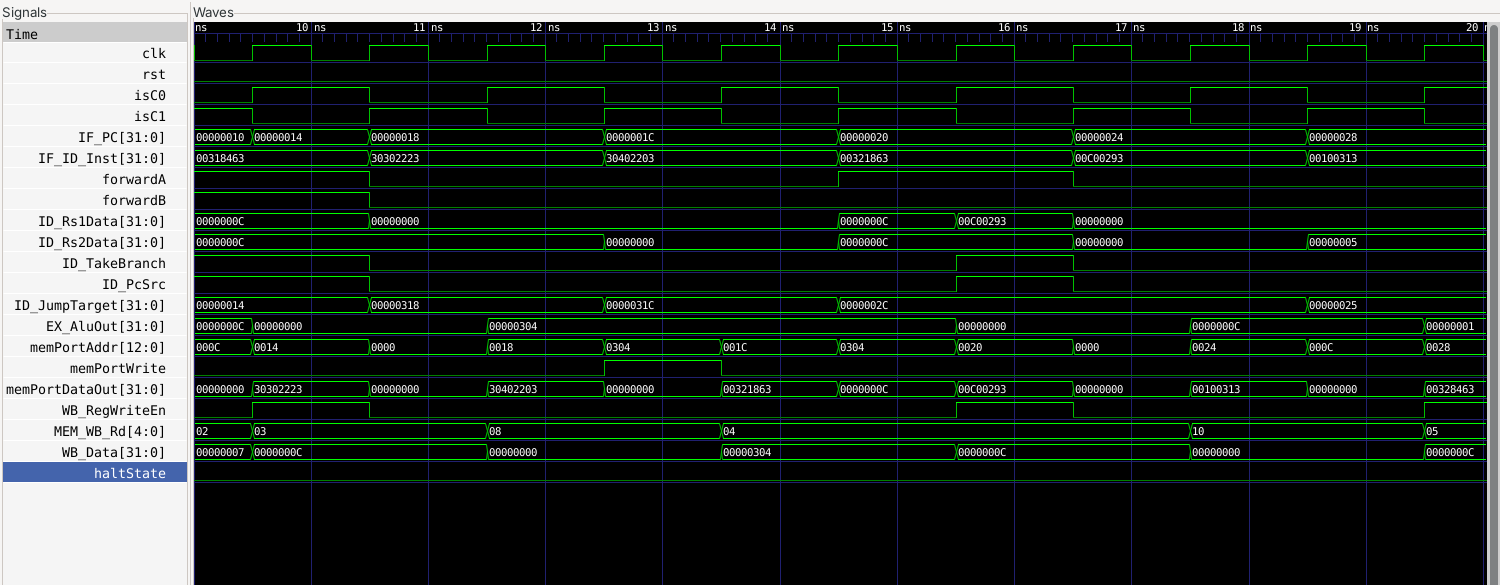
\includegraphics[width=\linewidth]{figures/wave_demo_hazard.png}
\caption{\file{demo} program, 9--20\,ns. \texttt{beq x3,x3} (\texttt{0x00318463}) directly follows \texttt{add x3,x2,x1}: both forwarding selects are high, both operands are \texttt{0xC}, \sig{ID_TakeBranch} rises in C1 and the next PC is the target \texttt{0x14}, so \texttt{0x10} is never fetched. Later \texttt{bne x4,x3} receives the load result of \texttt{lw x4} through \sig{forwardA} from the memory output; it is not taken.}
\end{figure}

\begin{figure}[H]\centering
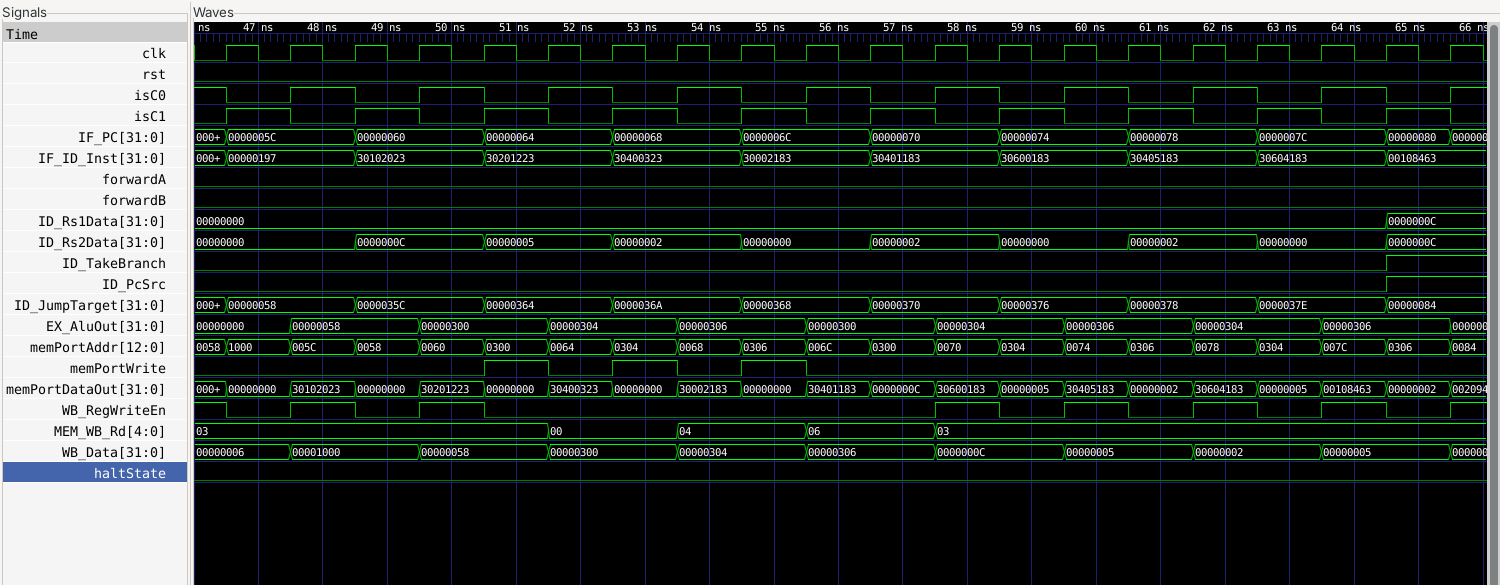
\includegraphics[width=\linewidth]{figures/wave_quick_memory.png}
\caption{\file{quick} program, 46--66\,ns: \texttt{sw}, \texttt{sh}, \texttt{sb} (three \sig{memPortWrite} pulses, always in C1, at \texttt{0x300}, \texttt{0x304}, \texttt{0x306}) followed by \texttt{lw}, \texttt{lh}, \texttt{lb}, \texttt{lhu}, \texttt{lbu}. The memory address alternates between PC (C0) and data address (C1).}
\end{figure}

\begin{figure}[H]\centering
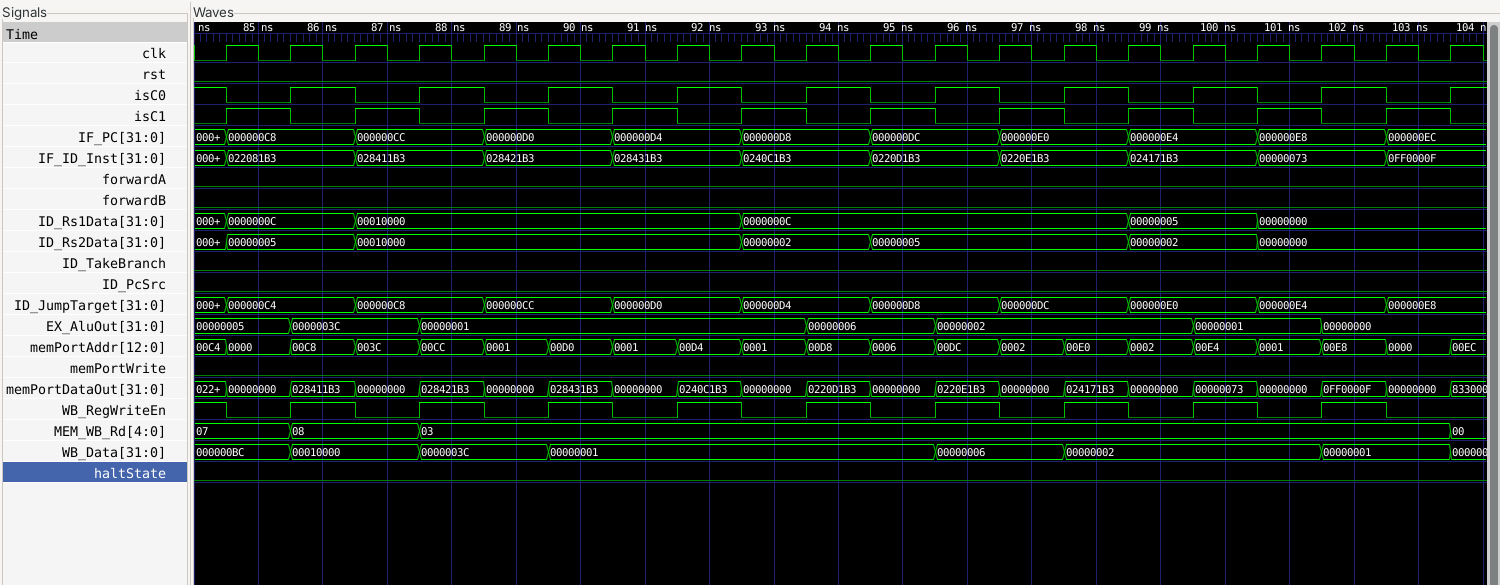
\includegraphics[width=\linewidth]{figures/wave_quick_muldiv.png}
\caption{\file{quick} program, 84--104\,ns: \texttt{lui} then \texttt{mul}, \texttt{mulh}, \texttt{mulhsu}, \texttt{mulhu}, \texttt{div}, \texttt{divu}, \texttt{rem}, \texttt{remu}; write-back values 60, 1, 1, 1, 6, 2, 2, 1.}
\end{figure}

\hd{5. FPGA testing (Nexys A7-100T)}

The top level (\file{datapath\_board\_pipelined.v}) uses BTNC as a debounced single-step CPU clock (one press = one cycle). SW15 is reset, SW0 chooses LED bits 14..0 or 30..16 of the instruction in ID, and SW3 SW2 SW1 choose what the 8-digit decimal display shows: 000 PC, 001 instruction in ID, 010 EX result, 011 memory address, 100 memory data, 101 store data, 110 write-back data, 111 write-back register. LD15 and the decimal points light when EBREAK has halted the CPU. The program \file{quick} executes every instruction once; \file{test/board\_quick\_guide.md} lists the expected value for every press.

The photos show the display in the write-back data view while stepping the first instructions of \file{quick}:

\begin{center}\small
\begin{tabular}{@{}c l c c@{}}
\toprule
Photo & Instruction & Press & Display\\
\midrule
(a) & \texttt{li x1, 12} & 4 & 00000012\\
(b) & \texttt{li x2, 5} & 6 & 00000005\\
(c) & \texttt{li x4, 2} & 8 & 00000002\\
(d) & \texttt{add x3, x1, x2} & 10 & 00000017\\
\bottomrule
\end{tabular}
\end{center}

\begin{figure}[H]\centering
\begin{subfigure}{0.48\linewidth}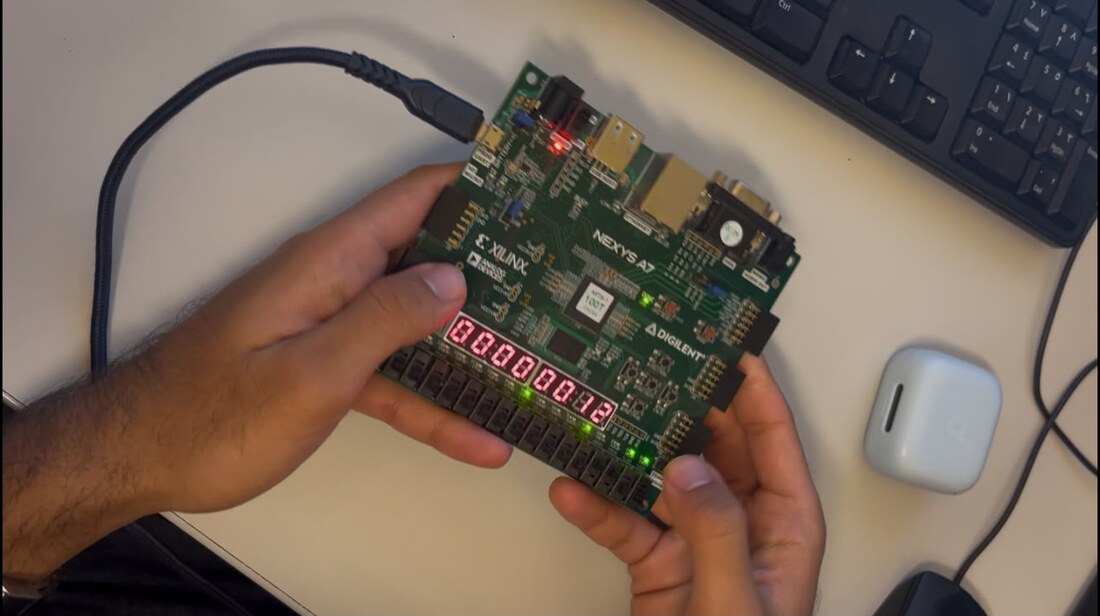
\includegraphics[width=\linewidth]{figures/board_display_12.jpg}\caption{12}\end{subfigure}\hfill
\begin{subfigure}{0.48\linewidth}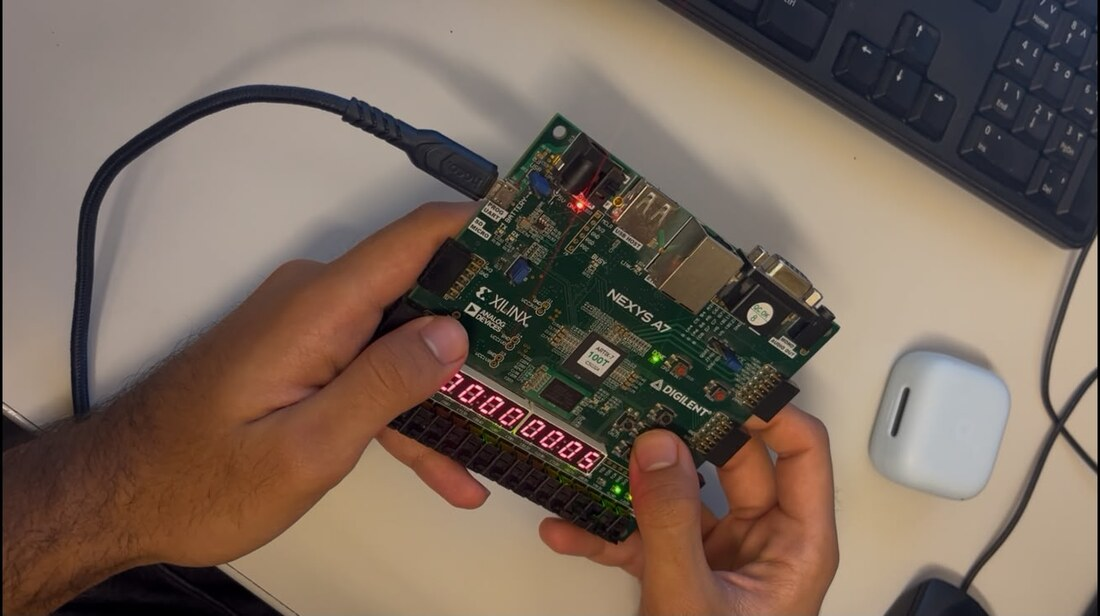
\includegraphics[width=\linewidth]{figures/board_display_5.jpg}\caption{5}\end{subfigure}\\[0.5em]
\begin{subfigure}{0.48\linewidth}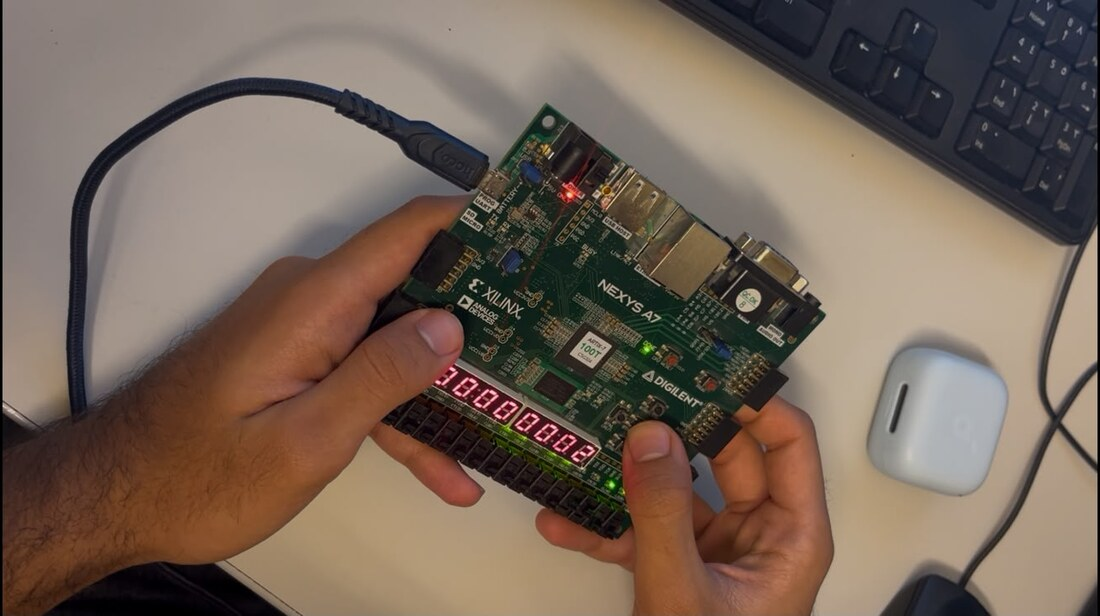
\includegraphics[width=\linewidth]{figures/board_display_2.jpg}\caption{2}\end{subfigure}\hfill
\begin{subfigure}{0.48\linewidth}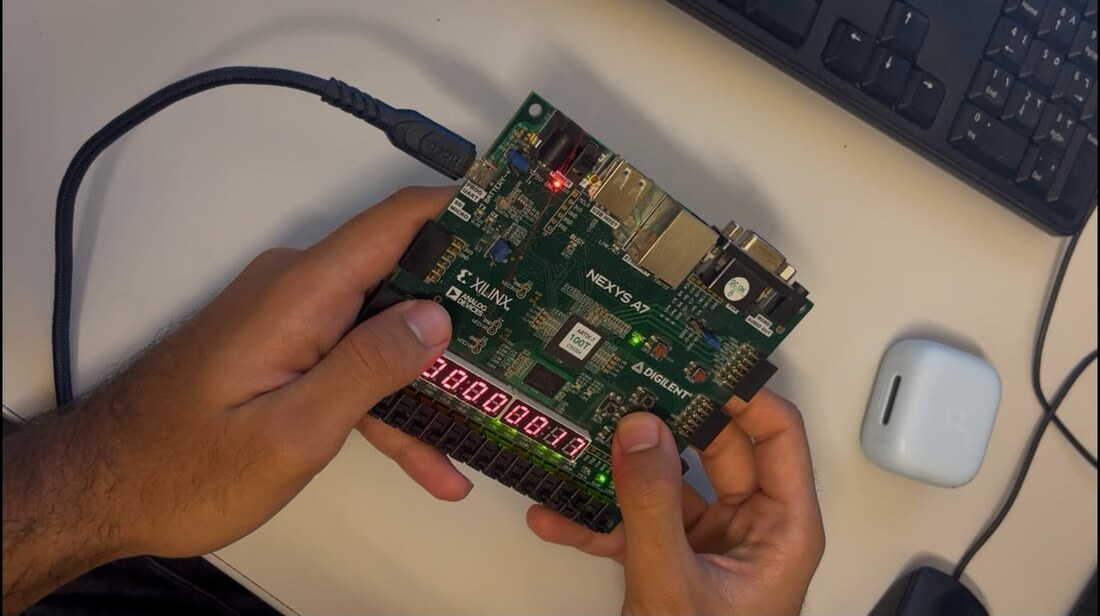
\includegraphics[width=\linewidth]{figures/board_display_17.jpg}\caption{17}\end{subfigure}
\caption{Display values on the board, matching the table above (the display is decimal).}
\end{figure}

\hd{6. Issues, assumptions and limitations}

\begin{center}\small
\begin{tabularx}{\linewidth}{@{}l X@{}}
\toprule
Issue & Solution\\
\midrule
One memory port for instructions and data & Two-cycle stages: IF uses the port in C0, MEM in C1 (CPI = 2)\\
Branches in EX cost two cycles; a hazard unit stalled for branch operands & Decision moved to ID with forwarding into ID: no penalty, no stalls, no flush except after EBREAK\\
Branch predictor (Bonus 3) draft & Dropped: with the decision in ID there is no misprediction cost to hide\\
Decode halted on ECALL as well as EBREAK & Only EBREAK halts; ECALL, FENCE, FENCE.TSO, PAUSE are NOPs\\
Memory should not use thousands of flip-flops & Word array with byte enables, mapped to distributed RAM\\
Vivado default simulation time is 1000\,ns & Testbench uses a 1\,ns clock and a built-in program; it ends at 485\,ns\\
\bottomrule
\end{tabularx}
\end{center}

\textbf{Limitations.} Loads and stores must be aligned (misaligned access and the \texttt{ma\_data} test are not supported). No traps, CSRs or FENCE.I. Memory is 1 KB (code from \texttt{0x000}, data from \texttt{0x300}). RV32M is combinational. The board is clocked by a button, so no maximum frequency is claimed.

\hd{7. Reproduce}

\begin{lstlisting}
cd Verilog
sh ../test/run_all.sh              # all simulations: PASS / FAIL
python3 ../test/mutation_test.py   # 8 / 8 mutants caught
cd ../test/wave && sh make_waves.sh   # VCD files for GTKWave
\end{lstlisting}
For Vivado: add all \file{Verilog/*.v} except testbenches, \file{defines.vh} and \file{const1.xdc}; top module \file{datapath_board_pipelined}.

\hd{8. AI disclosure}

Claude Pro and Gemini Pro were used.

\begin{center}\small
\begin{tabularx}{\linewidth}{@{}l X X@{}}
\toprule
Part of this report & What the AI did & Prompt used\\
\midrule
Datapath schematic (Fig.~\ref{fig:datapath}) & Wrote the TikZ drawing from the Verilog sources & ``Draw the datapath of this 3-stage pipeline from pipeline.v as TikZ, with the pipeline registers, the forwarding unit and the branch logic in ID, and the single memory shared by IF and MEM.''\\
Simulation results (Sec.~3) & Ran the testbench, riscv-tests, board programs and mutation test and collected the numbers & ``Run every self-checking test in the Verilog and test folders with Icarus Verilog and give me the pass counts.''\\
Waveform screenshots (Sec.~4) & Wrote a wrapper that dumps a VCD without editing the design, opened it in GTKWave and captured the screenshots; wrote the figure captions & ``Dump a VCD for the demo and quick programs without changing the Verilog, open it in GTKWave with the pipeline signals and take screenshots.''\\
Board table (Sec.~5) & Matched the four board photos to the expected values of the quick program & ``Which instruction and button press of the quick program produces each value shown on the board photos?''\\
Design check & We asked the assistants to check the connections and the hazard handling of the design and to report anything wrong & ``Check the connections between the modules in pipeline.v and the forwarding and branch hazard handling, and tell me if anything is wrong.''\\
Report wording and layout & Refined the wording of the text and the layout of the tables and figures & ``Tighten the wording of this report and improve the layout of the tables and figures without changing the content.''\\
\bottomrule
\end{tabularx}
\end{center}

\end{document}
